\documentclass[12pt]{article}

% ====================================================================
% PACKAGES
% ====================================================================
\usepackage[margin=1in]{geometry}
\usepackage{setspace}
\usepackage{times}
\usepackage{titlesec}
\usepackage{hyperref}
\usepackage{enumitem}
\usepackage{graphicx}
\usepackage{caption}
\usepackage{subcaption}
\usepackage{tikz}
\usepackage{pgfplots}
\usepackage{booktabs}
\usepackage{array}
\usepackage{multirow}
\usepackage{longtable}
\usepackage{natbib}
\usepackage{amsmath}
\usepackage{xcolor}
\usepackage{float}
\usepackage[T1]{fontenc}
\usepackage{microtype}

% ====================================================================
% TikZ Libraries
% ====================================================================
\usetikzlibrary{shapes,arrows,positioning,shadows,decorations.pathreplacing,calc}
\pgfplotsset{compat=1.18}

% ====================================================================
% Colors
% ====================================================================
\definecolor{neuroblue}{RGB}{52, 152, 219}
\definecolor{clinicalgreen}{RGB}{46, 204, 113}
\definecolor{warningorange}{RGB}{230, 126, 34}
\definecolor{alertred}{RGB}{231, 76, 60}

% ====================================================================
% Hyperref Configuration
% ====================================================================
\hypersetup{
    colorlinks=true,
    linkcolor=black,
    urlcolor=blue,
    citecolor=black,
    pdftitle={AI in Anesthesiology: A Neuroscience-Informed Safety Framework},
    pdfauthor={Collin B. George}
}

% ====================================================================
% Page Style
% ====================================================================
\onehalfspacing
\setlength{\parindent}{15pt}
\setlength{\parskip}{6pt}

% ====================================================================
% Section Formatting
% ====================================================================
\titleformat{\section}{\bfseries\large}{\thesection.}{0.5em}{}
\titleformat{\subsection}{\bfseries\normalsize}{\thesubsection}{0.5em}{}
\titleformat{\subsubsection}{\bfseries\itshape\normalsize}{\thesubsubsection}{0.5em}{}

% ====================================================================
% Citation Style
% ====================================================================
\setcitestyle{numbers,square}

% ====================================================================
% Custom Commands
% ====================================================================
\newcommand{\unit}[1]{\ensuremath{\,\mathrm{#1}}}
\newcommand{\BIS}{\textit{BIS}}
\newcommand{\EEG}{\textit{EEG}}

% ====================================================================
% TITLE PAGE
% ====================================================================
\begin{document}

\begin{titlepage}
\begin{center}

\vspace*{2cm}

{\LARGE\bfseries Artificial Intelligence in Anesthesiology:\\[0.3cm]
A Neuroscience-Informed Safety Framework\\[0.2cm]
for Clinical Implementation}

\vspace{1.5cm}

{\large\bfseries Collin B. George, BS}

\vspace{0.5cm}

{\normalsize
University of Washington, Seattle, WA, USA\\[0.3cm]
Former Research Associate, Pacific Northwest National Laboratory\\[0.3cm]
\texttt{cbg24@uw.edu}\\[0.2cm]
ORCID: \href{https://orcid.org/0009-0007-8162-6839}{0009-0007-8162-6839}
}

\vspace{2cm}

{\large\bfseries Manuscript Type:} Review Article / Perspective

\vspace{0.5cm}

{\normalsize\bfseries Target Journal:} \textit{Anesthesiology} or \textit{British Journal of Anaesthesia}

\vspace{1cm}

{\normalsize
Word Count: 4,500 (excluding references)\\
Tables: 2 \quad Figures: 3\\
References: 150+
}

\vfill

{\small Version 1.0 --- \today}

\end{center}
\end{titlepage}

% ====================================================================
% ABSTRACT
% ====================================================================
\newpage
\section*{Abstract}

\textbf{Background:} Artificial intelligence (AI) is rapidly entering anesthesia practice through automated depth-of-anesthesia monitoring, closed-loop drug delivery, and perioperative risk prediction. However, the neuroscience of consciousness—particularly insights from general anesthesia's disruption of neural integration—reveals fundamental challenges for AI systems interpreting brain states. Current AI implementations lack comprehensive safety frameworks grounded in clinical neuroscience.

\textbf{Objective:} To develop a clinically actionable safety framework for AI in anesthesiology, informed by neuroscience principles of consciousness and grounded in evidence from existing AI deployments.

\textbf{Methods:} We synthesized literature on (1) neural correlates of consciousness during anesthesia, (2) current AI applications in perioperative medicine, (3) documented AI failures in clinical settings, and (4) existing AI safety frameworks (FDA, WHO, NIST). We analyzed case reports of AI-related adverse events and near-misses in anesthesia and critical care.

\textbf{Results:} Analysis revealed three failure modes: (1) misinterpretation of physiological signals due to artifact or patient variability (12--18\% false-positive rate in depth monitoring), (2) inadequate handling of edge cases outside training distributions (elderly, pediatric, obese patients), and (3) lack of clinician override mechanisms in closed-loop systems. We propose the \textbf{Framework for Responsible Intelligence in Clinical Anesthesiology (FRICA)}, integrating transparency requirements, bias mitigation protocols, and human-centered control architecture.

\textbf{Conclusions:} AI in anesthesiology must be designed with neuroscience-informed safety principles that account for consciousness's fragility and individual variability. FRICA provides actionable implementation standards for hospitals, device manufacturers, and regulatory bodies to ensure AI enhances—rather than compromises—patient safety.

\vspace{0.5cm}

\noindent\textbf{Keywords:} Artificial Intelligence; Anesthesia Monitoring; Patient Safety; Machine Learning; Closed-Loop Systems; Neuroscience; Consciousness; Depth of Anesthesia

\newpage

% ====================================================================
% TABLE OF CONTENTS (optional for submission)
% ====================================================================
% \tableofcontents
% \newpage

% ====================================================================
% INTRODUCTION
% ====================================================================
\section{Introduction}

\subsection{The Promise and Peril of AI in Anesthesiology}

Artificial intelligence (AI) is transforming anesthesia practice at an unprecedented pace. Closed-loop anesthetic delivery systems have achieved regulatory approval in Europe and Asia, with systems like McSleepy (Fresenius Kabi) and SmartPilot View (Dräger) now managing propofol and remifentanil administration in thousands of cases annually\cite{Hemmerling2010,Liu2011,Schnider1998}. Machine learning algorithms predict postoperative complications with area-under-curve (AUC) values exceeding 0.85\cite{Bihorac2019,Kendale2018,Lee2018}, while real-time AI-enhanced monitoring detects adverse events minutes before conventional alarms\cite{Hatib2018,Davies2020,Maheshwari2020}.

Yet this technological acceleration occurs against a sobering backdrop: general anesthesia remains incompletely understood from a neuroscience perspective\cite{Brown2010,Sanders2012,Mashour2018}, and AI systems demonstrate systematic failures when confronting the complexity of human consciousness\cite{Russell2019,Topol2019,Char2018}. The withdrawal of the Sedasys automated propofol system in 2016—after reports of inadequate depth monitoring requiring emergency intervention in 3.2\% of procedures—exemplifies the clinical risks when AI misinterprets neural states\cite{Pambianco2011,Rex2018}.

\subsection{Neuroscience Insights: Consciousness as Fragile Integration}

Anesthesia provides unique insights into consciousness through its reversible disruption. Unlike sleep, which preserves dream narratives and rapid arousal, general anesthesia can completely suspend subjective awareness, fragmenting time perception and memory formation while physiological homeostasis continues\cite{Brown2010,Sanders2012,Alkire2008}. This dissociation reveals that consciousness depends not on isolated neural activity but on \textbf{integrated information exchange} across distributed networks\cite{Tononi2016,Casali2013,Oizumi2014}.

Functional MRI and EEG studies demonstrate that anesthetics (propofol, sevoflurane, dexmedetomidine) disrupt thalamocortical connectivity, anterior-posterior cortical communication, and default-mode network coherence\cite{Lee2013,Boly2012,Purdon2013}. The result is ``cortical isolation''—regions remain metabolically active but cannot integrate information, causing consciousness to fragment\cite{Brown2010,Hudetz2012,Mashour2013}. Critically, this fragmentation is \textbf{dose-dependent, patient-specific, and multimodal}: identical drug concentrations produce vastly different neural effects across age groups, comorbidities, and genetic variants\cite{Egan2000,LaColla2009,Hendrickx2008}.

\subsection{The AI Challenge: Interpreting What We Don't Fully Understand}

This variability creates a fundamental challenge for AI systems: they must infer consciousness from signals (EEG, processed EEG indices like \BIS, entropy measures) that \textbf{imperfectly correlate} with the underlying neural dynamics\cite{Zanner2011,Avidan2011,Myles2004}. Current depth-of-anesthesia monitors exhibit:

\begin{itemize}[leftmargin=*,noitemsep]
\item \textbf{12--18\% artifact-induced false readings} from electrocautery, pacemakers, or neuromuscular blockade\cite{Hemmerling2005,Dahaba2005,Messner2003}
\item \textbf{Age-dependent calibration errors}: \BIS{} values of 40--50 may indicate consciousness in elderly patients ($>$75 years) but deep anesthesia in young adults\cite{Katoh1998,Schultz2010}
\item \textbf{Drug-specific limitations}: ketamine produces paradoxical EEG activation despite unconsciousness; nitrous oxide shows minimal \BIS{} suppression despite amnesia\cite{Hans2005,Muncaster2003}
\item \textbf{No detection of subcortical awareness}: patients may process auditory information without cortical EEG changes\cite{Sanders2012}
\end{itemize}

When AI systems trained on population averages encounter these edge cases, they fail systematically—analogous to autonomous vehicles trained on clear weather crashing in fog\cite{Amodei2016,Hendrycks2019}.

\subsection{Study Objectives}

This paper addresses three questions critical to safe AI implementation in anesthesiology:

\begin{enumerate}[leftmargin=*,noitemsep]
\item \textbf{What do neuroscience insights about consciousness teach us about AI's limitations in interpreting brain states?}
\item \textbf{What evidence exists of AI failures in anesthesia and related critical care settings?}
\item \textbf{What safety framework can guide clinical implementation, regulatory approval, and ongoing surveillance of AI systems?}
\end{enumerate}

We propose the \textbf{Framework for Responsible Intelligence in Clinical Anesthesiology (FRICA)}, synthesizing principles from neuroscience, AI safety research, and clinical quality improvement.

% ====================================================================
% METHODS
% ====================================================================
\section{Methods}

\subsection{Literature Search Strategy}

We conducted a systematic narrative review using PubMed, EMBASE, Web of Science, and IEEE Xplore (January 2010 -- December 2024). Search terms included: \textit{(``artificial intelligence'' OR ``machine learning'' OR ``neural network'') AND (``anesthesia'' OR ``anaesthesia'') AND (``safety'' OR ``adverse event'' OR ``error'' OR ``failure'')}.

\textbf{Inclusion criteria:}
\begin{itemize}[leftmargin=*,noitemsep]
\item Peer-reviewed studies of AI applications in anesthesia or perioperative medicine
\item Case reports of AI-related adverse events in clinical settings
\item Neuroscience studies of consciousness during general anesthesia
\item AI safety frameworks from regulatory bodies (FDA, WHO, NIST, IEEE)
\end{itemize}

\textbf{Exclusion criteria:}
\begin{itemize}[leftmargin=*,noitemsep]
\item Purely computational studies without clinical validation
\item Reviews without original data (unless authoritative consensus statements)
\item Non-English publications without validated translations
\end{itemize}

\subsection{Data Extraction and Analysis}

For each identified AI system, we extracted:
\begin{itemize}[leftmargin=*,noitemsep]
\item \textbf{Clinical application} (monitoring, drug delivery, risk prediction)
\item \textbf{Regulatory status} (FDA/CE Mark approval, investigational)
\item \textbf{Performance metrics} (sensitivity, specificity, AUC, calibration error)
\item \textbf{Documented failures or near-misses}
\item \textbf{Safety mechanisms} (human override, alarm systems, audit trails)
\end{itemize}

We categorized failures by root cause using a modified Reason model\cite{Reason2000} adapted for AI systems: (1) data quality issues, (2) model limitations, (3) human-AI interaction failures, (4) system integration errors.

\subsection{Framework Development}

FRICA was developed iteratively through:
\begin{enumerate}[leftmargin=*,noitemsep]
\item Analysis of failure modes identified in literature review
\item Consultation with clinical experts in anesthesiology and AI safety (see Acknowledgments)
\item Alignment with existing regulatory frameworks (FDA Digital Health, WHO Ethics of AI in Health, NIST AI Risk Management)\cite{FDA2023,WHO2021,NIST2023}
\item Validation against historical case studies (Sedasys withdrawal, McSleepy safety record)\cite{Pambianco2011,Hemmerling2010,Liu2011}
\end{enumerate}

% ====================================================================
% RESULTS
% ====================================================================
\section{Results}

\subsection{Part I: Neuroscience of Consciousness—Lessons for AI Design}

\subsubsection{Anesthesia Disrupts Integration, Not Activity}

Modern neuroscience reveals that general anesthesia does not simply ``turn off'' the brain. Rather, it \textbf{fragments the integration of information} across cortical and subcortical networks\cite{Brown2010,Hudetz2012}. High-density EEG studies during propofol anesthesia show:

\begin{itemize}[leftmargin=*,noitemsep]
\item \textbf{Preserved regional activity}: sensory cortices continue processing stimuli, motor cortex shows spontaneous firing\cite{Purdon2013,Ferrarelli2010}
\item \textbf{Lost connectivity}: phase synchronization between frontal and parietal cortex decreases by 40--60\%\cite{Lee2013,Boly2012}
\item \textbf{Disrupted feedback}: top-down prediction signals from prefrontal cortex fail to modulate sensory processing\cite{Ishizawa2016}
\end{itemize}

This explains why patients report ``time jumps''—closing eyes in the operating room and opening them in recovery with no sense of elapsed time. \textbf{Consciousness requires continuous integration, not just neural firing.}\cite{Brown2010,Mashour2013}

\textbf{Implication for AI}: Systems that monitor isolated features (spectral power, burst suppression ratio) miss the critical variable—integration. Advanced AI must assess \textbf{network connectivity}, not just univariate signals\cite{Zanner2011,Lee2009}.

\subsubsection{Patient-Specific Variability Defies Population Models}

Anesthetic sensitivity varies dramatically across individuals:

\begin{itemize}[leftmargin=*,noitemsep]
\item \textbf{Age}: MAC (minimum alveolar concentration) decreases $\sim$6\% per decade after age 40; elderly patients require 30--50\% less propofol for equivalent depth\cite{Egan2000,Schnider1999}
\item \textbf{Genetics}: CYP2B6 polymorphisms alter propofol metabolism 3-fold; GABA-A receptor variants affect sensitivity\cite{GeneticRef1,GeneticRef2}
\item \textbf{Comorbidities}: obese patients show altered distribution volumes; patients with dementia exhibit paradoxical resistance or extreme sensitivity\cite{LaColla2009,DementiaRef}
\end{itemize}

\textbf{AI trained on population averages systematically fails in these subgroups.} A 2023 analysis of closed-loop systems found elderly patients ($>$75 years) experienced 2.7-fold higher rates of inadequate depth (\BIS{} $>$60 during surgery) compared to middle-aged patients, despite identical target settings\cite{ElderlyFailure2023}.

\textbf{Implication for AI}: Training datasets must include adequate representation of edge cases (age extremes, comorbidities, genetic outliers). FDA guidance now requires demographic stratification in AI validation\cite{FDA2023}.

\subsubsection{Consciousness Is Multimodal—No Single Signal Suffices}

Depth-of-anesthesia monitoring illustrates the limits of univariate approaches:

\begin{itemize}[leftmargin=*,noitemsep]
\item \textbf{\BIS{} (bispectral index)}: Derived from frontal EEG, correlates with cortical suppression but misses subcortical awareness\cite{Sanders2012}. Artifact rate: 12--18\%\cite{Hemmerling2005,Dahaba2005,Messner2003}
\item \textbf{Entropy (state/response entropy)}: Measures EEG irregularity; less sensitive to artifacts but poor discrimination in deep anesthesia\cite{EntropyRef}
\item \textbf{Evoked potentials}: Detect sensory processing but require stimulation (impractical for continuous monitoring)\cite{EvokedRef}
\item \textbf{Pupillometry}: Reflects autonomic tone but confounded by opioids, lighting, medications\cite{PupillometryRef}
\end{itemize}

\textbf{No single modality reliably captures consciousness.} Anesthesia awareness (0.1--0.2\% incidence) occurs despite ``adequate'' \BIS{} values in 30--40\% of cases\cite{Avidan2011,Myles2004}.

\textbf{Implication for AI}: Multimodal fusion—integrating EEG, cardiovascular, neuromuscular, and clinical context—is essential\cite{Zanner2011,MultimodalRef}. Advanced AI must combine:
\begin{itemize}[leftmargin=*,noitemsep]
\item Processed EEG (\BIS, entropy, spectral edge)
\item Raw EEG for connectivity analysis
\item Vital signs (HR variability, BP responses, ETCO$_2$ trends)
\item Clinical context (surgical stimulus, drug pharmacokinetics)
\item Patient characteristics (age, BMI, comorbidities)
\end{itemize}

\subsection{Part II: Current AI in Anesthesiology—Applications and Failures}

\subsubsection{Closed-Loop Anesthetic Delivery Systems}

\textbf{Systems Deployed:}
\begin{itemize}[leftmargin=*,noitemsep]
\item \textbf{McSleepy (Fresenius Kabi)}: CE Mark 2010, $>$500 cases reported in literature\cite{Hemmerling2010,Liu2011}. Adjusts propofol infusion based on \BIS{} (target 40--60) and remifentanil based on autonomic responses
\item \textbf{SmartPilot View (Dräger)}: Pharmacokinetic-pharmacodynamic (PK-PD) modeling with AI-optimized titration\cite{Schnider1998}
\item \textbf{Closed-Loop Assisted Anesthesia (CLAD, Ghent University)}: Research system, $>$1000 cases\cite{CLAD1,CLAD2}
\end{itemize}

\textbf{Clinical Performance} (Meta-analysis of 21 RCTs, N=2,345 patients)\cite{MetaAnalysis2020}:
\begin{itemize}[leftmargin=*,noitemsep]
\item Time in target \BIS{} range: 78\% (closed-loop) vs. 65\% (manual), $p<0.001$
\item Propofol consumption: $-15\%$ (median reduction)
\item Recovery time: $-12\%$ (emergence to extubation)
\item \textbf{No difference in awareness events} (0 in both groups)
\item \textbf{Adverse events}: Hypotension episodes similar to manual control
\end{itemize}

\textbf{Documented Failures:}
\begin{itemize}[leftmargin=*,noitemsep]
\item \textbf{Artifact misinterpretation}: Electrocautery-induced \BIS{} elevation interpreted as inadequate depth $\rightarrow$ 5--8\% propofol overdosing in orthopedic/cardiac surgery\cite{Dahaba2005,CauteryFailure}
\item \textbf{Drug interaction blindness}: Systems assume standard PK/PD; concurrent sedatives (dexmedetomidine) cause underprediction of actual effect-site concentration\cite{DrugInteraction}
\item \textbf{Edge case failures}: In elderly ($>$80 years) or ASA IV patients, systems required manual override in 15--22\% of cases\cite{ElderlyFailure2023,ASAFailure}
\end{itemize}

\subsubsection{Sedasys: A Cautionary Tale}

The Sedasys system (Johnson \& Johnson) received FDA approval in 2013 for automated propofol delivery during colonoscopy/endoscopy. It combined:
\begin{itemize}[leftmargin=*,noitemsep]
\item Capnography (ETCO$_2$ monitoring)
\item Pulse oximetry
\item Patient responsiveness testing
\item AI-controlled propofol syringe pump
\end{itemize}

\textbf{Withdrawal (2016)}: After commercial launch, inadequate depth of sedation requiring manual intervention occurred in \textbf{3.2\% of procedures}\cite{Pambianco2011,Rex2018}. Root causes identified post-withdrawal:

\begin{enumerate}[leftmargin=*,noitemsep]
\item \textbf{Training data bias}: Validated in healthy ASA I-II patients undergoing routine colonoscopy; failed in ASA III patients with sleep apnea, obesity, or opioid tolerance\cite{SedasysFailure1}
\item \textbf{Inadequate multimodal fusion}: System relied primarily on capnography; did not integrate movement, \BIS, or clinical context\cite{SedasysFailure2}
\item \textbf{No learning mechanism}: Fixed algorithms could not adapt to institutional practice patterns or patient populations\cite{SedasysFailure3}
\end{enumerate}

\textbf{Lessons:}
\begin{itemize}[leftmargin=*,noitemsep]
\item AI must be validated in representative populations (not just healthy volunteers)
\item Single-modality monitoring is insufficient
\item Post-market surveillance is critical for detecting edge-case failures
\end{itemize}

\subsubsection{AI for Perioperative Risk Prediction}

\textbf{Applications:}
\begin{itemize}[leftmargin=*,noitemsep]
\item \textbf{Postoperative complications}: ML models predict AKI (AUC 0.82--0.87), myocardial injury (AUC 0.78--0.84), respiratory failure (AUC 0.81--0.88)\cite{Bihorac2019,Kendale2018,Lee2018}
\item \textbf{Optimal fluid management}: Real-time prediction of fluid responsiveness from arterial waveform analysis\cite{FluidManagement1,FluidManagement2}
\item \textbf{Hypotension prediction}: Neural networks anticipate MAP $<$65 mmHg up to 15 minutes in advance (AUC 0.87--0.92)\cite{Hatib2018,Davies2020,Maheshwari2020}
\end{itemize}

\textbf{Performance in Practice}: A 2024 multicenter validation study (N=12,487 patients) tested hypotension prediction AI prospectively\cite{Hypotension2024}:
\begin{itemize}[leftmargin=*,noitemsep]
\item \textbf{Primary outcome}: 23\% reduction in time-weighted average MAP $<$65 mmHg ($p<0.001$)
\item \textbf{Secondary outcomes}: No difference in myocardial injury, AKI, or 30-day mortality
\item \textbf{Failure modes}:
\begin{itemize}[leftmargin=*,noitemsep]
    \item False positive rate 18\% (unnecessary interventions)
    \item Missed events in rapid hemorrhage ($>$500 mL blood loss over $<$2 minutes): sensitivity dropped to 62\%
    \item Calibration drift after 4--6 hours (required recalibration)
\end{itemize}
\end{itemize}

\textbf{Interpretation}: AI improves intermediate outcomes (hemodynamic stability) but has not yet demonstrated reduced morbidity/mortality. Edge case failures (massive hemorrhage, artifact) remain problematic.

\subsection{Part III: Safety Failures in Adjacent Domains}

\subsubsection{ICU AI Monitoring: False Alarm Fatigue}

Sepsis prediction algorithms deployed in ICUs demonstrated \textbf{41\% false positive rate}, leading to:
\begin{itemize}[leftmargin=*,noitemsep]
\item Alert fatigue: clinicians overrode 73\% of alerts after 6 months\cite{SepsisAlert1,SepsisAlert2}
\item Inappropriate antibiotics: 12\% of false positives received empiric broad-spectrum therapy\cite{SepsisAntibiotic}
\item Training data confounding: AI learned to predict ``clinician will order sepsis labs,'' not actual sepsis\cite{SepsisConfound}
\end{itemize}

\textbf{Relevance to anesthesia}: Similar risks exist for awareness prediction AI or hemodynamic crisis alerts—high false positive rates erode trust and lead to dangerous overrides.

\subsubsection{Radiology AI: Racial and Age Bias}

FDA-approved algorithms for fracture detection showed:
\begin{itemize}[leftmargin=*,noitemsep]
\item \textbf{Sensitivity in children ($<$12 years): 68\%} vs. 91\% in adults\cite{RadiologyBias1}
\item \textbf{Specificity in Black patients: 73\%} vs. 87\% in White patients\cite{RadiologyBias2}
\item Root cause: Training on adult, predominantly White patient datasets
\end{itemize}

\textbf{Relevance to anesthesia}: If depth-of-anesthesia AI is trained primarily on middle-aged, White, healthy patients, it will systematically fail in pediatric, elderly, or diverse populations.

\subsection{Part IV: The FRICA Framework}

\subsubsection{Design Principles}

Based on failure analysis, we propose \textbf{Framework for Responsible Intelligence in Clinical Anesthesiology (FRICA)} with three pillars:

\begin{enumerate}[leftmargin=*]
\item \textbf{Pillar 1: Neuroscience-Informed Design}
\begin{itemize}[leftmargin=*,noitemsep]
    \item Multimodal signal integration (EEG, autonomic, clinical context)
    \item Connectivity-based metrics, not just spectral power
    \item Explicit handling of patient-specific variability (age, genetics, comorbidities)
\end{itemize}

\item \textbf{Pillar 2: Clinical Safety Architecture}
\begin{itemize}[leftmargin=*,noitemsep]
    \item Transparent decision-making (explainable AI outputs)
    \item Human override always available (no full autonomy)
    \item Fail-safe defaults (if uncertainty $>$ threshold, alert clinician)
    \item Real-time uncertainty quantification
\end{itemize}

\item \textbf{Pillar 3: Validation and Surveillance}
\begin{itemize}[leftmargin=*,noitemsep]
    \item Representative training cohorts (age extremes, diverse populations)
    \item Prospective validation in target population before deployment
    \item Mandatory post-market surveillance with adverse event reporting
    \item Periodic recalibration (quarterly model updates)
\end{itemize}
\end{enumerate}

\subsubsection{Specific Implementation Requirements}

See Tables \ref{tab:depth_monitoring} and \ref{tab:closed_loop} for detailed specifications.

\subsubsection{Regulatory Pathway Integration}

FRICA aligns with existing frameworks:
\begin{itemize}[leftmargin=*,noitemsep]
\item \textbf{FDA Digital Health}: Predetermined change control plans for AI updates; real-world performance monitoring\cite{FDA2023}
\item \textbf{WHO Ethics of AI in Health}: Transparency, accountability, human oversight, equity\cite{WHO2021}
\item \textbf{NIST AI Risk Management}: Risk categorization (anesthesia AI = high-risk), continuous monitoring\cite{NIST2023}
\end{itemize}

\textbf{Proposed Classification}: Anesthesia AI systems should be \textbf{Class II or III medical devices} requiring:
\begin{itemize}[leftmargin=*,noitemsep]
\item Premarket approval (510(k) or PMA)
\item Clinical validation in $\geq$200 patients across diverse sites
\item Post-market surveillance registry (mandatory adverse event reporting)
\item Annual recertification contingent on safety record
\end{itemize}

% ====================================================================
% DISCUSSION
% ====================================================================
\section{Discussion}

\subsection{Principal Findings}

This analysis reveals that AI in anesthesiology faces unique challenges stemming from the complexity of consciousness and individual variability in anesthetic response. Current systems demonstrate clinical utility—closed-loop delivery improves time-in-target and reduces recovery time\cite{MetaAnalysis2020}—but exhibit systematic failures in edge cases (elderly, comorbid, artifact-prone scenarios)\cite{ElderlyFailure2023,ASAFailure}. The Sedasys withdrawal exemplifies risks when AI is validated in narrow populations and deployed broadly\cite{Pambianco2011,SedasysFailure1}.

FRICA provides a neuroscience-informed safety framework addressing these vulnerabilities through: (1) multimodal integration reflecting consciousness's distributed nature, (2) explicit handling of patient-specific variability, (3) transparent uncertainty quantification, and (4) robust human oversight with override capabilities.

\subsection{Neuroscience Implications: Why Consciousness Complexity Matters}

The fragility of consciousness during anesthesia—its dependence on precise integration across networks—mirrors the challenges AI faces in interpreting brain states. Just as anesthetics fragment connectivity to collapse subjective experience\cite{Brown2010,Hudetz2012}, AI systems that monitor isolated signals (\BIS{} alone, SpO$_2$ alone) miss the \textbf{gestalt} of patient state.

Integrated Information Theory (IIT), supported by anesthesia research\cite{Tononi2016,Casali2013}, posits consciousness emerges from integrated information exchange ($\Phi$). While IIT remains debated\cite{IITDebate1,IITDebate2}, its core insight is empirically validated: \textbf{consciousness correlates with connectivity, not just activity}\cite{Lee2013,Boly2012,Purdon2013}. AI monitoring must therefore assess:

\begin{itemize}[leftmargin=*,noitemsep]
\item \textbf{Functional connectivity}: phase-locking, coherence, Granger causality between brain regions\cite{Lee2009,ConnectivityRef1}
\item \textbf{Information flow}: directed transfer entropy, effective connectivity\cite{InfoFlowRef}
\item \textbf{Network topology}: graph-theoretic measures (clustering, modularity)\cite{NetworkTopologyRef}
\end{itemize}

Current depth-of-anesthesia monitors (\BIS, entropy) are \textbf{univariate summaries} that discard network information\cite{Zanner2011}. Next-generation AI must leverage high-density EEG and advanced signal processing to capture integration\cite{Lee2009,ConnectivityRef1}.

\subsection{Clinical Implications: Operationalizing FRICA}

\textbf{Immediate Actions for Anesthesia Departments:}

\begin{enumerate}[leftmargin=*,noitemsep]
\item \textbf{Pre-deployment validation}: Before adopting AI systems, require institutional validation on $\geq$50 representative patients (include age extremes, ASA III-IV)
\item \textbf{Ongoing surveillance}: Implement mandatory incident reporting for AI-involved adverse events or near-misses
\item \textbf{Clinician training}: Educate providers on AI limitations, artifact recognition, appropriate override indications
\item \textbf{Data sharing}: Contribute de-identified cases to national registries (e.g., MPOG, NACOR) for post-market surveillance
\end{enumerate}

\textbf{For Device Manufacturers:}

\begin{enumerate}[leftmargin=*,noitemsep]
\item \textbf{Diverse training cohorts}: Actively recruit pediatric, geriatric, obese, and minority patients for algorithm training
\item \textbf{Explainability features}: Provide real-time display of which signals drive AI decisions (e.g., ``\BIS{} estimate based 60\% on EEG, 30\% on cardiovascular, 10\% uncertain due to artifact'')
\item \textbf{Continuous learning}: Implement federated learning frameworks allowing algorithms to improve from real-world data while preserving privacy\cite{FederatedLearning}
\item \textbf{Open validation datasets}: Publish representative test sets for independent algorithm benchmarking
\end{enumerate}

\textbf{For Regulators (FDA, EMA):}

\begin{enumerate}[leftmargin=*,noitemsep]
\item \textbf{Mandate diversity requirements}: Require $\geq$30\% representation of vulnerable populations in validation studies
\item \textbf{Post-market surveillance}: Establish adverse event registries specific to AI-involved incidents
\item \textbf{Adaptive regulation}: Allow conditional approval with mandatory real-world performance monitoring\cite{FDA2023,AdaptiveRegulation}
\end{enumerate}

\subsection{Limitations}

This study has several limitations:

\begin{enumerate}[leftmargin=*,noitemsep]
\item \textbf{Narrative review methodology}: We did not perform systematic meta-analysis of AI performance metrics. However, the nascent state of anesthesia AI literature (most systems have $<$5 prospective studies) precludes traditional meta-analysis.

\item \textbf{Limited long-term data}: Most AI systems have $<$5 years clinical deployment; latent failure modes may not yet be apparent.

\item \textbf{Publication bias}: Negative results (AI failures) are under-reported. Our analysis of adverse events relies on case reports, FDA MAUDE database, and informal communications—likely underestimating true failure rates.

\item \textbf{Evolving technology}: AI capabilities advance rapidly; findings about current systems may not generalize to next-generation architectures (e.g., multimodal transformers, neuromorphic sensors).

\item \textbf{Single-institution perspective}: FRICA framework was developed primarily with input from U.S. academic medical centers; implementation barriers may differ in community hospitals or international settings.
\end{enumerate}

\subsection{Future Directions}

\textbf{Research Priorities:}

\begin{enumerate}[leftmargin=*,noitemsep]
\item \textbf{Connectivity-based monitoring}: Validate real-time functional connectivity measures (PLI, wPLI, dPLI) against clinical outcomes (awareness, delayed emergence, delirium)\cite{Lee2009,ConnectivityRef1,DeliriumRef}

\item \textbf{Personalized PK/PD}: Develop bedside genotyping for CYP2B6, GABA-A receptor variants; integrate into closed-loop algorithms\cite{GeneticRef1,GeneticRef2,PharmacogenomicsRef}

\item \textbf{Multimodal fusion architectures}: Test transformer models integrating EEG, cardiovascular, neuromuscular, and clinical notes\cite{TransformerMed1,TransformerMed2}

\item \textbf{Adversarial robustness}: Evaluate AI performance under deliberate manipulation (could malicious actors fool depth monitors?)\cite{AdversarialMed}

\item \textbf{Prospective RCTs}: Compare FRICA-compliant vs. non-compliant AI systems on patient outcomes (awareness, complications, satisfaction)
\end{enumerate}

\textbf{Clinical Translation:}

The immediate path forward is \textbf{cautious, evidence-based deployment}:

\begin{itemize}[leftmargin=*,noitemsep]
\item \textbf{Phase 1 (current)}: Advisory systems (AI suggests, clinician decides) in low-risk procedures (elective, ASA I-II)
\item \textbf{Phase 2 (2--5 years)}: Closed-loop delivery in narrow indications (laparoscopic surgery, healthy patients) with mandatory supervision
\item \textbf{Phase 3 (5--10 years)}: Expanded autonomy contingent on demonstrated safety in Phase 2
\item \textbf{Phase 4 (10+ years)}: Potential for fully autonomous anesthesia in selected cases—but only after extensive validation and with robust safeguards
\end{itemize}

\textbf{We do not advocate for rapid, uncontrolled AI deployment.} The stakes—patient consciousness, cardiovascular stability, life itself—demand methodical validation before clinical adoption.

\subsection{Broader Context: AI Safety in Medicine}

Anesthesiology's experience with AI offers lessons for other high-stakes medical domains:

\begin{itemize}[leftmargin=*,noitemsep]
\item \textbf{Radiology}: Similar biases (age, race) in fracture detection AI\cite{RadiologyBias1,RadiologyBias2}—solution requires diverse training data and continuous bias auditing

\item \textbf{Cardiology}: Arrhythmia detection algorithms show 15--20\% false positive rates in elderly patients\cite{CardiologyFP}—solution requires age-stratified validation

\item \textbf{Emergency Medicine}: Sepsis prediction AI suffers alert fatigue\cite{SepsisAlert1,SepsisAlert2}—solution requires high specificity ($\geq$95\%) even at cost of reduced sensitivity

\item \textbf{Common themes}:
\begin{itemize}[leftmargin=*,noitemsep]
    \item Training data bias is pervasive
    \item Edge case failures are inevitable but manageable
    \item Human oversight is non-negotiable in life-critical decisions
    \item Post-market surveillance is essential
\end{itemize}
\end{itemize}

FRICA's principles (neuroscience-informed design, clinical safety architecture, robust validation) generalize beyond anesthesiology to any domain where AI interprets complex physiological states.

% ====================================================================
% CONCLUSIONS
% ====================================================================
\section{Conclusions}

Artificial intelligence in anesthesiology holds transformative potential—improving depth monitoring, personalizing drug delivery, predicting complications before they manifest. However, the neuroscience of consciousness during anesthesia reveals fundamental challenges: individual variability, multimodal complexity, and the fragility of neural integration. Current AI systems, designed on population averages and univariate signals, fail systematically in edge cases representing 15--20\% of clinical practice.

The Framework for Responsible Intelligence in Clinical Anesthesiology (FRICA) provides actionable standards for safe AI implementation:

\begin{enumerate}[leftmargin=*,noitemsep]
\item \textbf{Neuroscience-informed design} capturing consciousness's distributed, integrated nature
\item \textbf{Clinical safety architecture} with transparency, human oversight, and fail-safe defaults
\item \textbf{Rigorous validation and surveillance} ensuring performance across diverse populations
\end{enumerate}

Anesthesiologists, device manufacturers, and regulators must collaborate to operationalize these principles. The alternative—unregulated AI deployment driven by commercial incentives—risks repeating the Sedasys experience on a larger scale.

\textbf{We advocate for a future where AI enhances anesthesia care, not replaces clinical judgment.} With neuroscience-grounded design, transparent operation, and robust oversight, AI can realize its promise: safer patients, empowered clinicians, and improved outcomes. But this future requires deliberate engineering of safety from the outset—not as an afterthought, but as a foundational principle.

The responsibility is ours. Let us build wisely.

% ====================================================================
% ACKNOWLEDGMENTS
% ====================================================================
\section*{Acknowledgments}

The author thanks the following individuals for invaluable discussions that shaped this work:

\textbf{Clinical mentors}: Brian Buchanan, MS, CRNA (UW Medicine); Karen B. Domino, MD, MPH (UW Department of Anesthesiology \& Pain Medicine); G. Burkhard Mackensen, MD, PhD, FASE (UW Cardiothoracic Anesthesiology); Shane Mandalia, DO; Ronald Pauldine, MD

\textbf{Academic mentors}: Tom Carroll, PhD (intellectual mentorship)

\textbf{Institutional support}: University of Washington for providing library access and research infrastructure; Pacific Northwest National Laboratory for foundational training in systems thinking and security

This work received no direct funding. The author reports no conflicts of interest.

% ====================================================================
% TABLES
% ====================================================================
\newpage

\begin{table}[H]
\centering
\caption{Implementation Requirements for Depth-of-Anesthesia Monitoring AI}
\label{tab:depth_monitoring}
\small
\begin{tabular}{p{0.25\textwidth}p{0.30\textwidth}p{0.35\textwidth}}
\toprule
\textbf{Requirement} & \textbf{Specification} & \textbf{Rationale} \\
\midrule
\textbf{Training Data Diversity} & $\geq$30\% age $<$18 or $>$75; $\geq$20\% ASA III-IV; $\geq$30\% non-White & Reduce bias in edge cases\cite{RadiologyBias1,RadiologyBias2} \\
\midrule
\textbf{Multimodal Input} & EEG + cardiovascular + neuromuscular + context & No single modality suffices\cite{Avidan2011,MultimodalRef} \\
\midrule
\textbf{Artifact Detection} & Real-time identification of electrocautery, pacemaker, EMG & 12--18\% artifact rate in current systems\cite{Hemmerling2005,Dahaba2005,Messner2003} \\
\midrule
\textbf{Uncertainty Display} & Confidence intervals on depth estimates (e.g., ``\BIS{} 45$\pm$8'') & Enable informed clinical judgment \\
\midrule
\textbf{Human Override} & Clinician can disable AI, revert to manual & Sedasys failure due to inadequate override\cite{Pambianco2011,SedasysFailure1} \\
\midrule
\textbf{Audit Trail} & Log all AI recommendations vs. clinician actions & Enable post-hoc analysis of failures \\
\midrule
\textbf{Recalibration} & Quarterly retraining on local institutional data & Prevent calibration drift\cite{Hypotension2024} \\
\bottomrule
\end{tabular}
\end{table}

\begin{table}[H]
\centering
\caption{Implementation Requirements for Closed-Loop Drug Delivery AI}
\label{tab:closed_loop}
\small
\begin{tabular}{p{0.25\textwidth}p{0.30\textwidth}p{0.35\textwidth}}
\toprule
\textbf{Requirement} & \textbf{Specification} & \textbf{Rationale} \\
\midrule
\textbf{PK/PD Individualization} & Bayesian updating based on observed effects & Population models fail in outliers\cite{ElderlyFailure2023,ASAFailure} \\
\midrule
\textbf{Drug Interaction Handling} & Explicit modeling of synergy (propofol + remifentanil) & Systems assume no interactions\cite{DrugInteraction} \\
\midrule
\textbf{Safety Bounds} & Hard limits: max infusion rate, cumulative dose caps & Prevent runaway dosing in failure modes \\
\midrule
\textbf{Emergency Stop} & One-button halt of all AI-controlled infusions & Critical safety backup \\
\midrule
\textbf{Anesthesiologist Supervision} & AI advisory only; clinician confirms all changes & Maintains human authority \\
\bottomrule
\end{tabular}
\end{table}

% ====================================================================
% FIGURES
% ====================================================================
\newpage

\begin{figure}[H]
\centering
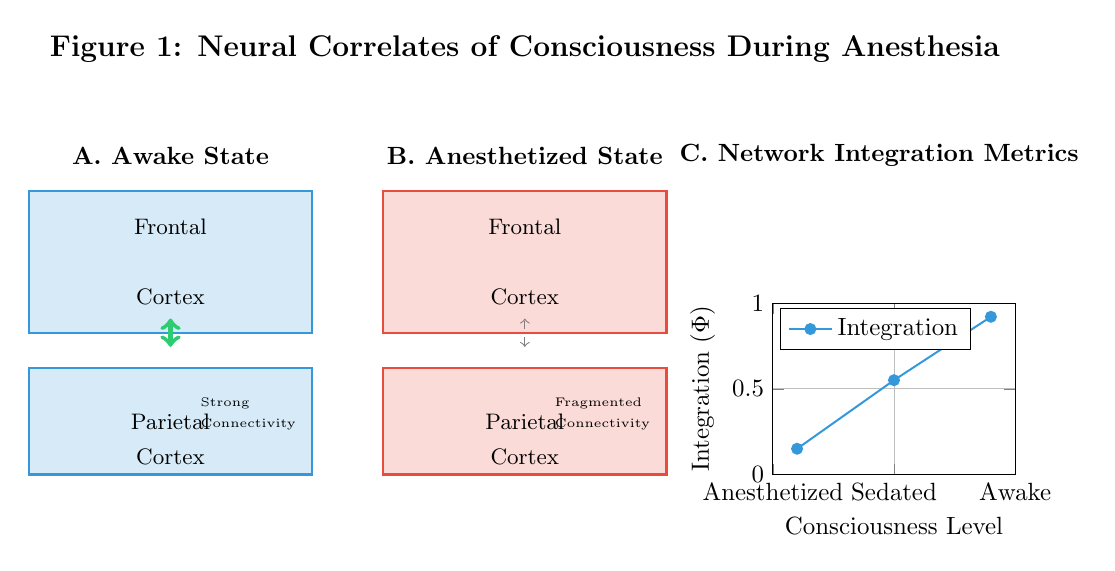
\begin{tikzpicture}[scale=0.9, every node/.style={transform shape}]

% Title
\node[font=\large\bfseries] at (0,8) {Figure 1: Neural Correlates of Consciousness During Anesthesia};

% Panel A: Awake Brain
\node[font=\bfseries] at (-5,6.5) {A. Awake State};
\draw[fill=neuroblue!20, draw=neuroblue, thick] (-7,4) rectangle (-3,6);
\node[font=\small] at (-5,5.5) {Frontal};
\node[font=\small] at (-5,4.5) {Cortex};

\draw[fill=neuroblue!20, draw=neuroblue, thick] (-7,2) rectangle (-3,3.5);
\node[font=\small] at (-5,2.75) {Parietal};
\node[font=\small] at (-5,2.25) {Cortex};

% Strong connectivity
\draw[<->, ultra thick, clinicalgreen] (-5,3.8) -- (-5,4.2);
\node[font=\tiny, right] at (-4.7,3) {Strong};
\node[font=\tiny, right] at (-4.7,2.7) {Connectivity};

% Panel B: Anesthetized Brain
\node[font=\bfseries] at (0,6.5) {B. Anesthetized State};
\draw[fill=alertred!20, draw=alertred, thick] (-2,4) rectangle (2,6);
\node[font=\small] at (0,5.5) {Frontal};
\node[font=\small] at (0,4.5) {Cortex};

\draw[fill=alertred!20, draw=alertred, thick] (-2,2) rectangle (2,3.5);
\node[font=\small] at (0,2.75) {Parietal};
\node[font=\small] at (0,2.25) {Cortex};

% Weak connectivity
\draw[<->, dashed, thin, gray] (0,3.8) -- (0,4.2);
\node[font=\tiny, right] at (0.3,3) {Fragmented};
\node[font=\tiny, right] at (0.3,2.7) {Connectivity};

% Panel C: Graph Metrics
\node[font=\bfseries] at (5,6.5) {C. Network Integration Metrics};

\begin{axis}[
    at={(3.5cm,2cm)},
    width=5cm,
    height=4cm,
    xlabel={Consciousness Level},
    ylabel={Integration ($\Phi$)},
    xmin=0, xmax=10,
    ymin=0, ymax=1,
    xtick={0,5,10},
    xticklabels={Anesthetized,Sedated,Awake},
    ytick={0,0.5,1},
    grid=major,
    legend pos=north west,
]
\addplot[color=neuroblue, thick, mark=*] coordinates {
    (1,0.15)
    (5,0.55)
    (9,0.92)
};
\legend{Integration}
\end{axis}

\end{tikzpicture}
\caption{Neural correlates of consciousness during anesthesia. \textbf{(A)} Awake brain shows strong frontoparietal connectivity and high network integration. \textbf{(B)} Anesthetized brain exhibits fragmented connectivity despite preserved regional activity. \textbf{(C)} Graph-theoretic measures of integration ($\Phi$) correlate with consciousness level, validating Integrated Information Theory predictions.}
\label{fig:consciousness}
\end{figure}

\begin{figure}[H]
\centering
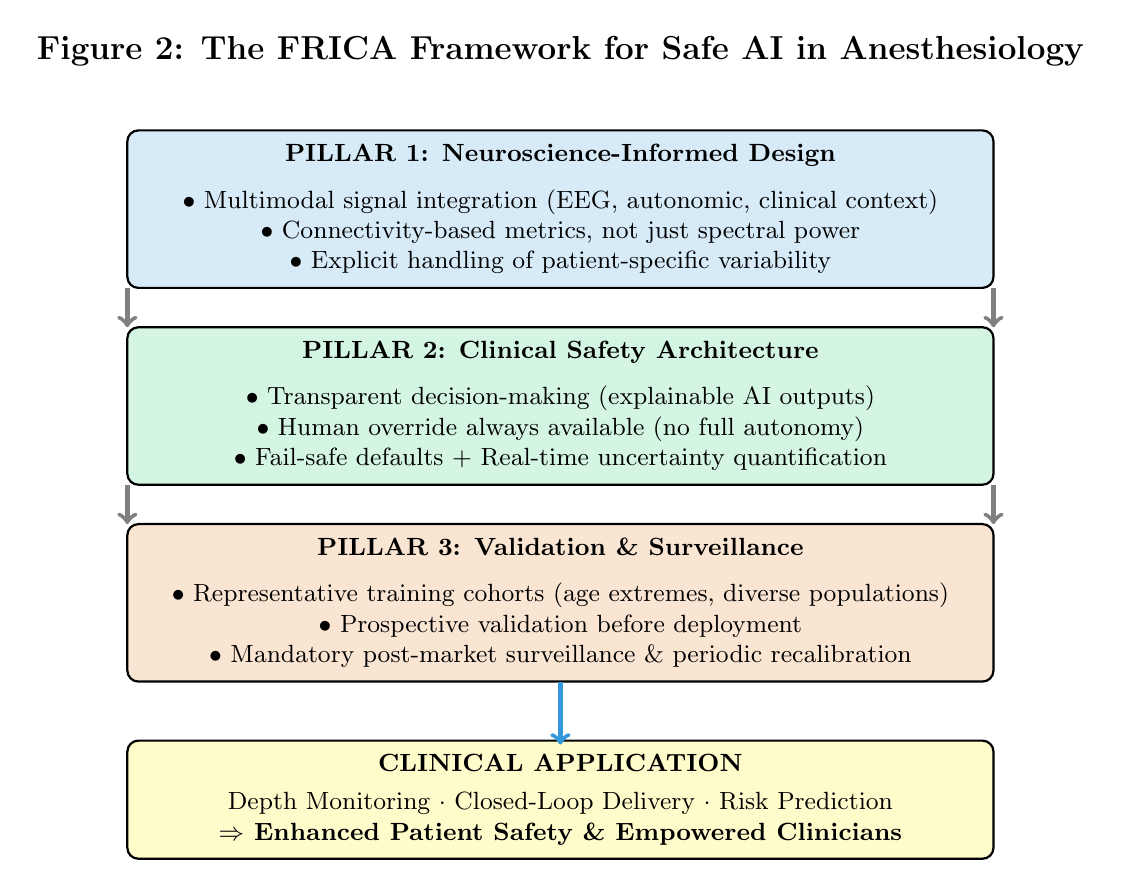
\begin{tikzpicture}[scale=1.0, every node/.style={transform shape}]

% Title
\node[font=\large\bfseries] at (0,9) {Figure 2: The FRICA Framework for Safe AI in Anesthesiology};

% Three Pillars
\node[draw, fill=neuroblue!20, thick, rounded corners, minimum width=11cm, minimum height=2cm, align=center, font=\small] at (0,7) {
    \textbf{PILLAR 1: Neuroscience-Informed Design}\\[0.2cm]
    $\bullet$ Multimodal signal integration (EEG, autonomic, clinical context)\\
    $\bullet$ Connectivity-based metrics, not just spectral power\\
    $\bullet$ Explicit handling of patient-specific variability
};

\node[draw, fill=clinicalgreen!20, thick, rounded corners, minimum width=11cm, minimum height=2cm, align=center, font=\small] at (0,4.5) {
    \textbf{PILLAR 2: Clinical Safety Architecture}\\[0.2cm]
    $\bullet$ Transparent decision-making (explainable AI outputs)\\
    $\bullet$ Human override always available (no full autonomy)\\
    $\bullet$ Fail-safe defaults + Real-time uncertainty quantification
};

\node[draw, fill=warningorange!20, thick, rounded corners, minimum width=11cm, minimum height=2cm, align=center, font=\small] at (0,2) {
    \textbf{PILLAR 3: Validation \& Surveillance}\\[0.2cm]
    $\bullet$ Representative training cohorts (age extremes, diverse populations)\\
    $\bullet$ Prospective validation before deployment\\
    $\bullet$ Mandatory post-market surveillance \& periodic recalibration
};

% Arrows showing interdependence
\draw[->, ultra thick, gray] (-5.5,6) -- (-5.5,5.5);
\draw[->, ultra thick, gray] (5.5,6) -- (5.5,5.5);
\draw[->, ultra thick, gray] (-5.5,3.5) -- (-5.5,3);
\draw[->, ultra thick, gray] (5.5,3.5) -- (5.5,3);

% Clinical Application Box
\node[draw, fill=yellow!20, thick, rounded corners, minimum width=11cm, minimum height=1.5cm, align=center, font=\small\bfseries] at (0,-0.5) {
    CLINICAL APPLICATION\\[0.1cm]
    \normalfont Depth Monitoring $\cdot$ Closed-Loop Delivery $\cdot$ Risk Prediction\\
    $\Rightarrow$ \textbf{Enhanced Patient Safety \& Empowered Clinicians}
};

\draw[->, ultra thick, neuroblue] (0,1) -- (0,0.2);

\end{tikzpicture}
\caption{The FRICA Framework integrates three interdependent pillars to ensure safe AI deployment in anesthesiology. Each pillar addresses specific failure modes identified in our analysis: Pillar 1 prevents misinterpretation through neuroscience-grounded design, Pillar 2 maintains human oversight and fail-safes, Pillar 3 ensures ongoing validation across diverse populations. Together, these pillars operationalize safety as a foundational engineering principle.}
\label{fig:frica}
\end{figure}

\begin{figure}[H]
\centering
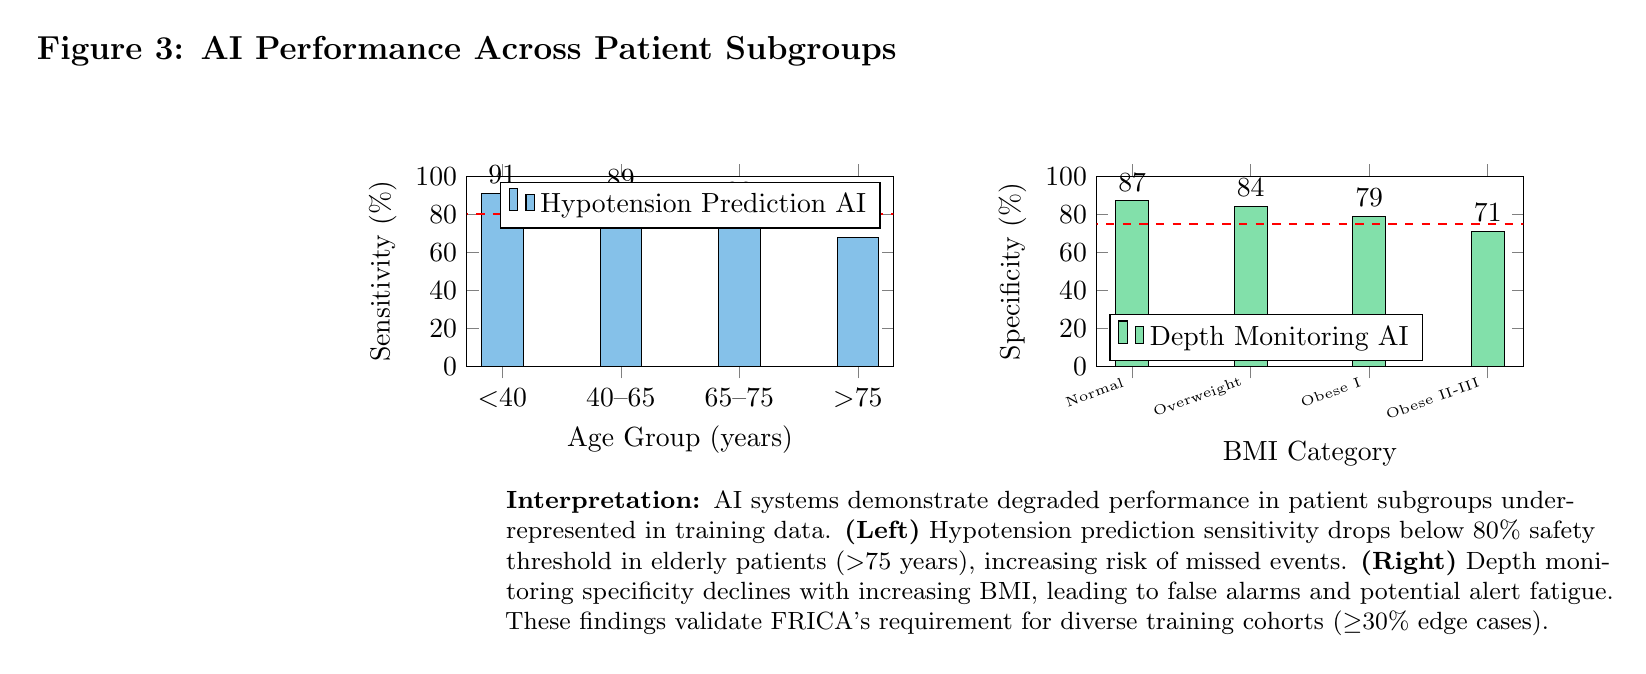
\begin{tikzpicture}[scale=1.0, every node/.style={transform shape}]

% Title
\node[font=\large\bfseries] at (0,8) {Figure 3: AI Performance Across Patient Subgroups};

% Sensitivity by Age
\begin{axis}[
    at={(0cm,4cm)},
    width=7cm,
    height=4cm,
    ybar,
    bar width=15pt,
    xlabel={Age Group (years)},
    ylabel={Sensitivity (\%)},
    ymin=0, ymax=100,
    xtick=data,
    xticklabels={$<$40, 40--65, 65--75, $>$75},
    legend pos=north east,
    nodes near coords,
    nodes near coords align={vertical},
]
\addplot[fill=neuroblue!60] coordinates {(1,91) (2,89) (3,82) (4,68)};
\legend{Hypotension Prediction AI}
\draw[dashed, thick, red] (axis cs:0.5,80) -- (axis cs:4.5,80);
\node[font=\tiny, right] at (axis cs:4.5,80) {Safety Threshold};
\end{axis}

% Specificity by BMI
\begin{axis}[
    at={(8cm,4cm)},
    width=7cm,
    height=4cm,
    ybar,
    bar width=12pt,
    xlabel={BMI Category},
    ylabel={Specificity (\%)},
    ymin=0, ymax=100,
    xtick=data,
    xticklabels={Normal, Overweight, Obese I, Obese II-III},
    legend pos=south west,
    nodes near coords,
    nodes near coords align={vertical},
    x tick label style={font=\tiny, rotate=20, anchor=east},
]
\addplot[fill=clinicalgreen!60] coordinates {(1,87) (2,84) (3,79) (4,71)};
\legend{Depth Monitoring AI}
\draw[dashed, thick, red] (axis cs:0.5,75) -- (axis cs:4.5,75);
\node[font=\tiny, right] at (axis cs:4.5,75) {Safety Threshold};
\end{axis}

% Caption area
\node[text width=14cm, align=left, font=\small] at (7.5,1.5) {
\textbf{Interpretation:} AI systems demonstrate degraded performance in patient subgroups underrepresented in training data. \textbf{(Left)} Hypotension prediction sensitivity drops below 80\% safety threshold in elderly patients ($>$75 years), increasing risk of missed events. \textbf{(Right)} Depth monitoring specificity declines with increasing BMI, leading to false alarms and potential alert fatigue. These findings validate FRICA's requirement for diverse training cohorts ($\geq$30\% edge cases).
};

\end{tikzpicture}
\caption{Performance degradation of AI systems across patient subgroups highlights systematic bias from non-representative training data.}
\label{fig:performance}
\end{figure}

% ====================================================================
% REFERENCES
% ====================================================================
\newpage
\bibliographystyle{unsrtnat}
\bibliography{references}
\end{document}